\section{Skaitmeninės tapatybės valdymo apžvalga}

Skaitmeniniame amžiuje tapatybės valdymas internete
yra svarbi taikomųjų programų dalis. Šiame skyriuje apžvelgiamas asmenų identifikavimo internete poreikis,
skaitmeninės tapatybės valdymo samprata, taikomi tapatybės valdymo modeliai bei pagrindinės naudotojams
kylančios problemos. Skaitmeninės tapatybės, autentifikavimo, autorizavimo bei kitų darbe
naudojamų terminų aiškinimai pateikiami skyriuje \enquote{Sąvokų apibrėžimai}.

\subsection{Tapatybės atpažinimo poreikis}

Naudotojo identifikavimas yra reikšminga interneto taikomųjų
programų dalis. Paslaugų tiekėjai identifikuoja savo naudotojus norėdami \cite{RalucaBudiu2014}:

\begin{itemize}
    \item registruoti (angl. \textit{log}) naudotojų veiklą,
    \item užtikrinti, kad naudotojas iš tikrųjų yra asmuo, kuris sakosi esąs,
    \item suteikti dalį funkcionalumo tik autorizuotiems naudotojams,
    \item individualizuoti tinklalapio ar taikomosios programos turinį pagal naudotojo poreikius,
    \item sukurti paslaugos naudotojų bendruomenę,
    \item išvengti galimų anoniminių naudotojų atakų.
\end{itemize}

Dėl išvardytų priežasčių naudotojų identifikavimas atlieka svarbią rolę įvairiose taikomųjų programų
srityse - elektroninėje valdžioje, elektroninėje komercijoje, verslo sumanume
(angl. \textit{business intelligence}), tyrimuose bei saugume
(angl. \textit{homeland security}) \cite{Glasser2009}. Kiekvienas paslaugų tiekėjas turi pasirinkti,
kaip autentifikuoti, ir, jei reikia, autorizuoti naudotojus. Programos kūrėjas taip pat turi užtikrinti naudotojo
suteiktų duomenų saugumą, o naudotojui tenka rūpintis skirtingų turimų
paskyrų priežiūra ir savo duomenų sklaida tarp skirtingų sistemų. Minimus tapatybės atpažinimo
skaitmeninėje erdvėje aspektus nagrinėja skaitmeninės tapatybės valdymo disciplina.

\subsection{Skaitmeninės tapatybės valdymo samprata}

Dėl nuolat vykstančios interneto ir jame esančių paslaugų plėtros tapatybių
valdymo uždavinys pastaraisiais metais tapo itin svarbus \cite{Glasser2009}. Skaitmeninės tapatybės valdymo pagrindinis uždavinys yra kontroliuoti
tapatybę ir su ja susijusius procesus, tokius kaip autentifikavimas, autorizavimas, prieigų kontrolė,
tapatybės gyvavimo ciklo valdymas bei saugus tapatybės atributų perdavimas trečiosioms šalims \cite{Cao2010, Dabrowski2008}. Sprendžiant šį uždavinį,
sukurta skirtingų skaitmeninės tapatybės valdymo sistemų. Šioms sistemoms įtaką daro
kiti tapatybę nagrinėjantys mokslai (pvz. sociologija), taip pat jos gali atlikti keletą skirtingų funkcijų, susijusių
su naudotojų tapatybe. Žemiau pateikiama diagrama,
kurioje apibendrintas tapatybės valdymo sistemų kontekstas bei pagrindinės atliekamos užduotys:

\begin{figure}[H]
    \centering
    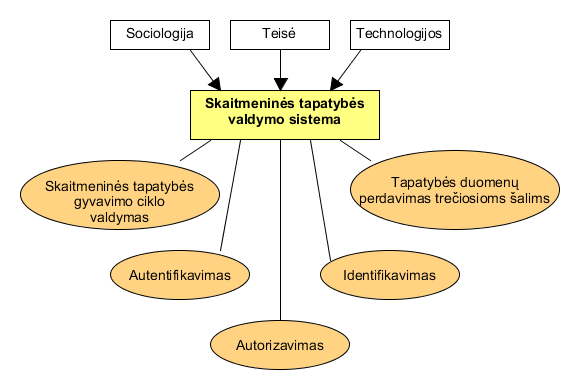
\includegraphics[scale=0.8]{img/IDMcontextAndUsecases}
    \caption{Skaitmeninių tapatybių valdymo sistemų kontekstas ir užduotys \cite{Glasser2009}}
    \label{fig:IDMContext}
\end{figure}

Paveiksle matomos disciplinos turi skirtingą poveikį tapatybių valdymo sistemoms. 
Sociologija padeda apibrėžti tapatybę ir jos atitikmenį skaitmeninėje erdvėje, teisės mokslas nusako tapatybės duomenų naudojimo reikalavimus,
o esamos technologijos formuoja sistemos įgyvendinimo niuansus. Verta pastebėti, kad tapatybės valdymo sistema gali atlikti ne visas
diagramoje nurodomas funkcijas, o tik dalį iš jų.

\subsection{Naudotojų poreikiai skaitmeninės tapatybės valdymo sistemoms} \label{section:IDMUserNeeds}

Skaitmeninės tapatybės valdymas yra plati sritis, kurią galima analizuoti iš skirtingų pusių: paslaugų tiekėjo, tapatybės tiekėjo ar naudotojo.
Šiame darbe į skaitmeninių tapatybių valdymą žvelgta iš naudotojo perspektyvos - kaip skaitmeninio valdymo sistemos atitinka naudotojų poreikius
bei lūkesčius. Išskirtos šios naudotojoms aktualios sistemų savybės:

\begin{itemize}
    \item atpažinimo duomenų kiekis. Naudotojui vidutiniškai turint 25 paskyras, reikalaujančias slaptažodžių \cite{Florencio2007} bei naudojant
    nuo 2 iki 12-os el. paštų \cite{Gross2007}, jis tampa priverstas prisiminti vis daugiau slaptažodžių bei identifikatorių. Atsimintinų autentifikavimo duomenų kiekiui
    augant, naudotojai yra linkę aukoti saugumą dėl patogumo ir naudoti panašius
    slaptažodžius skirtingose sistemose \cite{Pashalidis2003, Samar1999};
    \item saugumas. Privatumas yra žmogaus poreikis ir visa visuomenė nukentėtų nuo jo nebuvimo \cite{Maliki2007}.
    Suteikiant savo asmens duomenis internete naudotojai tikisi, kad jie bus patikimai
    saugomi ir nepasiekiami programišiams. Tapatybių valdymo sistemos turėtų būti budrios saugumo rizikoms bei viešai skelbti
    saugumui skirtas priemones ir atliktų saugumo analizių rezultatus, kad tiek naudotojai, tiek paslaugų tiekėjai
    galėtų pasitikėti tapatybių valdymo sistemomis \cite{Dhamija2008};
    \item asmens duomenų kontrolė. Pasak Nyderlanduose atliktų tyrimų, naudotojai nesijaučia kontroliuojantys savo asmens duomenų internete \cite{Baars2016}. Dėl to
    naudotojai pradeda nepasitikėti taikomųjų programų kūrėjais, nes jie pilnai nežino, kokia informacija apie juos kaupiama ir kokioms
    sistemoms ji perduodama;
    \item patogumas (angl. \textit{usability}). Naudotojams skaitmeninės tapatybės valdymas neretai yra tik pašalinis mechanizmas, reikalingas
    norint pasiekti paslaugą \cite{Dhamija2008}. Dėl šios priežasties sistemos naudojimosi patogumas yra svarbus - kuo tapatybės valdymas yra labiau integruotas
    su asmens jau naudojamomis sistemomis, kuo mažiau jis reikalauja papildomo naudotojo įsitraukimo ir kuo suteikia geresnę naudotojo patirtį (angl. \textit{user experience}), tuo labiau naudotojas bus linkęs pasirinkti šį identiteto valdymo sprendimą.
\end{itemize}

\subsection{Skaitmeninės tapatybės valdymo modeliai}

Naudojamų tapatybių valdymo sistemų architektūros bei veikimo principai yra skirtingi. S. Clauß ir M.Köhntopp savo tyrime pastebi,
kad nėra vieningo standarto identiteto valdymo sistemoms \cite{Claus2001}. Šiame skyriuje tiriami 3-ys dažniausiai naudojami identiteto valdymo
modeliai. Tiriant kiekvieną modelį, pirmiausia apžvelgti jo bendri veikimo principai. Taip pat apžvelgtos paplitusios modelį įgalinančios technologijos
(angl. \textit{enabling technology}),
nes modelio realizacijoje taikomi standartai ar protokolai gali turėti įtakos naudotojų poreikiams. Galiausiai, analizuotas modelio atitikimas naudotojų lūkesčiams,
išvardytiems \hypertarget{section:IDMUserNeeds}{~\ref{section:IDMUserNeeds}} skyrelyje.

\subsubsection{Izoliuotas tapatybių valdymas}

\subsubsubsection*{Modelis}

Izoliuotame modelyje paslaugų tiekėjas yra ir tapatybės tiekėjas, nes visos su tapatybės valdymu
susijusios operacijos yra atliekamos vieno serverio. Tapatybės duomenų saugojimas, autentifikavimas
ir autorizavimas yra įgyvendinti paties paslaugų tiekėjo \cite{Cao2010}. Kiekvienas naudotojas turi atskirus identifikatorius
kiekvienai naudojamai paslaugai. Modelis grafiškai pavaizduotas žemiau esančiame paveiksle.

\begin{figure}[H]
    \centering
    \includegraphics[scale=0.65]{img/IsolatedModel}
    \caption{Izoliuotas skaitmeninės tapatybės valdymas \cite{Cao2010}}
\end{figure}

Pagal izoliuotą modelį, naudotojas turi savo paskyrą kiekvienoje naudojamoje sistemoje. Kiekvieną kartą autentifikuojant ar autorizuojant
naudotoją, tai atlieka pats paslaugų tiekėjas, bendraudamas tiesiogiai su naudotoju (jo naršykle). Naudotojui prisijungus prie vieno tinklalapio ir gavus
prieigos raktą, jis gali toliau naudotis šiuo tinklalapiu, tačiau prireikus pasinaudoti kita taikomąja programa, tapatybės atpažinimo veiksmai (autentifikavimas, autorizavimas)
turi vėl būti atlikti naujoje sistemoje.

\subsubsubsection*{Realizacijos bei įgalinančios technologijos}

Kadangi šis naudotojų autentifikavimo bei autorizavimo modelis naudojamas seniausiai,
yra gana nemažai jį įgyvendinusių taikomųjų programų. Apsilankius keleto įmonių
interneto tinklalapiuose, pastebėta, kad Lietuvoje naują paskyrą susikurti siūlo
\enquote{Tiketa}, \enquote{Bilietai.lt}, \enquote{Pigu.lt},
\enquote{Varle.lt}, pasaulyje - \enquote{Booking.com}, \enquote{Skycop}, \enquote{AirBnB}, \enquote{CodinGame} bei kitos platformos (išvardytų
įmonių puslapiai tikrinti 2018 metų balandžio 14-ą dieną). Dalis iš jų remiasi ne vien tik savo izoliuotu tapatybės valdymu,
bet jau turi į savo sistemas integravę ir papildomų autentifikavimo būdų
(pvz. prisijungimą per \enquote{Facebook} ar \enquote{Google}).

Realizacijų technologiniai sprendimai dažniausiai nėra viešai prieinami.
Šiame modelyje kiekvienas paslaugų tiekėjas yra ir tapatybės tiekėjas, tad nereikia
apibrėžti protokolų, duomenų formatų ar kitų detalių, kurios formalizuotų bendravimą tarp pasikliaujančiosios šalies ir
tapatybės tiekėjo - visa tai pats nusprendžia ir įgyvendina paslaugų tiekėjas.

\subsubsubsection*{Naudotojų poreikių įgyvendinimas}

Nors izoliuotas tapatybių valdymas yra gana paprastas paslaugų tiekėjams, tačiau jis greitai tampa
nebekontroliuojamu naudotojams \cite{Josang2005}. Jis verčia naudotojus turėti paskyrą kiekvienai paslaugai, o tai lemia
daugybės identifikatorių ir slaptažodžių valdymą. Tai sukelia \enquote{slaptažodžių nuovargį} (angl. 
\textit{password fatigue}), o tai veda prie tų pačių identifikatorių ir slaptažodžių pasirinkimo skirtingoms paslaugoms \cite{Dhamija2008}.

Izoliuotame identiteto valdyme programišiams sunkiau atlikti sukčiavimo (angl. \textit{phishing}) ataką, nes naudotojas
nebūna nukreipiamas į tapatybės tiekėjo puslapį. Tai pagerina šio modelio saugumą. Dėl to, kad paslaugų tiekėjas yra ir tapatybės tiekėjas,
šiame modelyje galima išvengti duomenų perdavimo tarp skirtingų serverių - tokiu būdu sumažėja ir rizika, kad šiuos duomenis
jų persiuntimo metu perims programišius. Tačiau, standartų duomenų formatams bei perdavimui nebuvimas gali paskatinti paslaugų
tiekėjus nepažvelgti į tai atsakingai ir įgyvendinti bendravimą su naudotojo naršykle atmestinai.

Naudotojų asmens duomenų kontrolė šiame modelyje priklauso nuo kiekvienos paslaugos. Asmenys atskirai suteikia savo duomenis
kiekvienai paslaugai, dažniausiai paskyros sukūrimo metu. Jei paslauga informuoja apie duomenų panaudos atvejus (pvz. kam bus naudojamas
el. pašto adresas), tuomet asmuo jausis labiau užtikrintas savo duomenų kontrole. Tačiau dėl šiame modelyje neišvengiamo duomenų suteikimo
dideliam skirtingų paslaugų kiekiui, asmeniui tampa sunku prisiminti kiekvienos naudojamos platformos duomenų platinimo taisykles.

Izoliuotame tapatybės valdyme naudotojams tenka kartoti identifikavimo procesus (autentifikavimą, autorizavimą) tiek kartų, kiek paslaugų siekiama
naudotis. Tai vargina naudotojus ir kuria blogą naudotojo patirtį. Tačiau, izoliuotas tapatybės valdymas pasižymi nuoseklia vartotojo sąsaja (dėl 
visų tapatybės valdymo procesų įgyvendimo tame pačiame paslaugų tiekėjo puslapyje), tad tai šiek tiek pagerina bendrą naudotojo patirtį.

\subsubsection{Centralizuotas tapatybių valdymas}

\subsubsubsection*{Modelis}
Centralizuotame skaitmeninių tapatybių valdyme egzistuoja vienas tapatybės tiekėjas, į kurį kreipiasi visos paslaugos,
esančios to paties paslaugų tiekėjo domene \cite{Josang2005}. Kai paslaugų tiekėjui
reikia autentifikuoti naudotoją (ar atlikti kitą tapatybės valdymo procesą), jis persiųs naudotojo pateiktus atpažinimo duomenis tapatybės tiekėjui,
siekdamas pabaigti procesą \cite{Cao2010}. Naudotojui šiame modelyje užtenka vienų atpažinimo duomenų, su kuriais jis gali prisijungti prie visų to paties
paslaugų tiekėjo paslaugų. Modelio veikimas iliustruotas \hypertarget{fig:centralisedModel}{~\ref{fig:centralisedModel}}-iame paveiksle.

\begin{figure}[H]
    \centering
    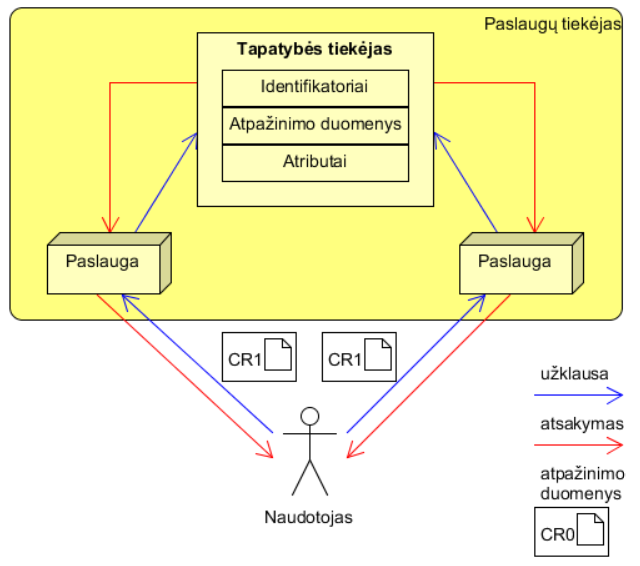
\includegraphics[scale=0.8]{img/centralizedModel}
    \caption{Centralizuotas skaitmeninės tapatybės valdymas \cite{Cao2010}}
    \label{fig:centralisedModel}
\end{figure}

Centralizuotame modelyje paslaugų tiekėjo ir tapatybės tiekėjo funkcijos tampa atskirtos - 
tapatybės tiekėjas rūpinasi naudotojo identiteto valdymu, o paslaugų tiekėjas koncentruojasi į paslaugos vystymą. Tai sudaro patrauklesnes sąlygas
naudotojui, tačiau taip pat sukuria vieno nesekmės taško (angl. \textit{single point of failure}) sistemą. Tapatybės tiekėjo sistemai tapus nepasiekiamai,
naudotojai nebegali naudotis nei viena paslauga tame pačiame domene.

\subsubsubsection*{Realizacijos bei įgalinančios technologijos}

Centralizuotas modelis tinkamiausias naudoti darbuotojams įmonės ribose arba vieno paslaugų tiekėjo paslaugoms \cite{Josang2005}.
Pateikiami pavyzdžiai abiems šioms realizacijoms. 

Viena iš įmonėse naudojamų realizacijų centralizuotam tapatybės valdymui - 
katalogų prieigos protokolas (angl. \textit{Lightweight Directory Access Protocol}, toliau LDAP), naudojamas pasiekti ir palaikyti informaciją interneto tinkle \cite{Strictest2011}.
Šis protokolas dažniausiai sujungiamas su aktyviąja direktorija (angl. \textit{active directory}) ir leidžia laikyti kompanijos darbuotojų
tapatybės informaciją vienoje vietoje. Taikomosios programos siunčia užklausas į LDAP serverį, kuriose nurodo norimą atlikti veiksmą (pvz. naudotojo
autentifikavimą ar naudotojo atributų atnaujinimą). Informacija per LDAP perduodama LDAP duomenų apsikeitimo formatu (LDIF).\\
LDAP grįstas vienkartinis prisijungimas leidžia įmonės darbuotojams vieną kartą prisijungti prie tam tikros įmonėje naudojamos programos ir
nebekartoti prisijungimo kreipiantis į kitą programą. Tačiau, tai galios tik toms programoms, kurios pasiekiamoms darbuotojams per vidinį intranetą
\cite{Strictest2011}. Dėl šios priežasties LDAP grįstas centralizuotas tapatybės valdymas retai sutinkamas už įmonių intraneto ribų \cite{Strictest2011}.

Centralizuotas tapatybės valdymas taip pat gali būti realizuotas ir ne įmonės ribose, jei konkretus paslaugų tiekėjas
turi keletą paslaugų, skirtų naudotojams. Tokiu atveju jis gali turėti centralizuotą posistemę tapatybės valdymui, o naudotojui užtenka
turėti vieną paslaugų tiekėjo paskyrą visoms įmonės paslaugoms. Tokios realizacijos pavyzdys - \enquote{Atlassian} įmonės paslaugos. Naudotojui pakanka turėti vieną \enquote{Atlassian} paskyrą ir jis gali naudotis
skirtingais šio paslaugų tiekėjo produktais, tokiais kaip \enquote{Jira}, \enquote{Confluence}, \enquote{Bitbucket} bei kitais. Vieną kartą prisijungus prie \enquote{Atlassian} programos (pvz. \enquote{Jira}),
naudotojas tampa autentifikuotas ir kituose \enquote{Atlassian} tinklalapiuose. 

\subsubsubsection*{Naudotojų poreikių įgyvendinimas}
 
Iš naudotojo perspektyvos, centralizuotas modelis yra patogesnis nei izoliuotas. Naudotojui pakanka turėti vienus atpažinimo duomenis,
kurie bus tinkami visoms konkretaus paslaugų tiekėjo programoms. Tačiau, norint pasiekti kito paslaugų tiekėjo paslaugą,
naudotojo turima paskyra nebebus tinkama.

Centralizuotas tapatybės valdymas ne intranete gali patirti sukčiavimo (angl. \textit{phishing}) ataką, jei paslaugų tiekėjas nukreipinėja naudotoją į tinklalapį kitame domene. Tačiau,
kadangi paslaugų tiekėjas tapatybės valdymą realizuoja pats, jis gali leisti naudotojui vesti identifikavimo duomenis ir pačiame paslaugos puslapyje (o ne nukreipiant
į kitą sistemą) arba nukreipti į tame pačiame domene esantį, paties paslaugų tiekėjo valdomą puslapį. Tai sumažina sukčiavimo jautrumo (angl. \textit{phishing susceptibility}) galimybę.

Naudotojai neturi didelės asmens duomenų kontrolės centralizuotame tapatybės valdyme. Nors, skirtingai nei izoliuotame modelyje, jie suteikia duomenis mažesniam kiekiui taikomųjų programų
(nebe kiekvienai programai, o kiekvienam paslaugų tiekėjui), tačiau tai vis dar nėra ideali situacija. Naudotojams vistiek reikia kontroliuoti
visas skirtingų paslagų tiekėjų paskyras ir žinoti su jomis susijusias duomenų saugojimo bei platinimo taisykles. Taip pat, jeigu modelis taikomas ne įmonės intranete (kur
duomenų apsikeitimui apibrėžtas formatas, pvz. LDIF), naudotojas nežino, kokiu būdu jo prisijungimo ar kiti duomenys bus perduodami iš vienos paslaugos į kitą.

Centralizuotas tapatybės valdymo modelis sudaro palankias sąlygas gerai naudotojo patirčiai užtikrinti. Centralizuotas modelis, priklausomai nuo realizacijos,
gali palaikyti vienkartinį prisijungimą, o tai leidžia naudotojui prisijungti vieną kartą ir tapti autentifikuotu visose paslaugų tiekėjo sistemose. Taip pat, kadangi
tiek tapatybės valdymo, tiek paslaugų puslapiai yra valdomi paties paslaugų tiekėjo, gali būti užtikrintas vientisas tinklalapių stilius. Taigi, centralizuotą tapatybės valdymą
įgyvendinę paslaugų tiekėjai gali sukurti patogias, naudotojams draugiškas (angl. \textit{user-friendly}) sistemas.

\subsubsection{Jungtinis tapatybių valdymas}


\subsubsubsection*{Modelis}

Ilgą laiką centralizuoto tapatybių valdymo pakako įmonėms turėti patogų, pačios įmonės prižiūrimą tapatybės valdymo sprendimą. Tačiau augant 
naudojamų taikomųjų programų bei integracijų su trečiųjų šalių aplikacijomis kiekiui, reikėjo sprendimo, leidžiančio identiteto valdymo uždavinius
spręsti ne tik vienos organizacijos ribose. Todėl buvo pradėtas naudoti jungtinis (angl. \textit{federated}) tapatybių valdymas.

Jungtinis (angl. \textit{federated}) tapatybių valdymas yra aibė technologijų
ir procesų, kurie leidžia sistemoms dalintis tapatybės informacija ir deleguoti tapatybės valdymo užduotis
tarp skirtingų paslaugų tiekėjų \cite{Maler2008}. Šis tapatybių valdymo modelis įgalina naudotojus turėti vienus atpažinimo duomenis,
kuriuos gali naudoti skirtingų paslaugų tiekėjų tinklalapiuose. Žemiau pateikiama schema, vaizduojanti
šio modelio architektūrą:

\begin{figure}[H]
    \centering
    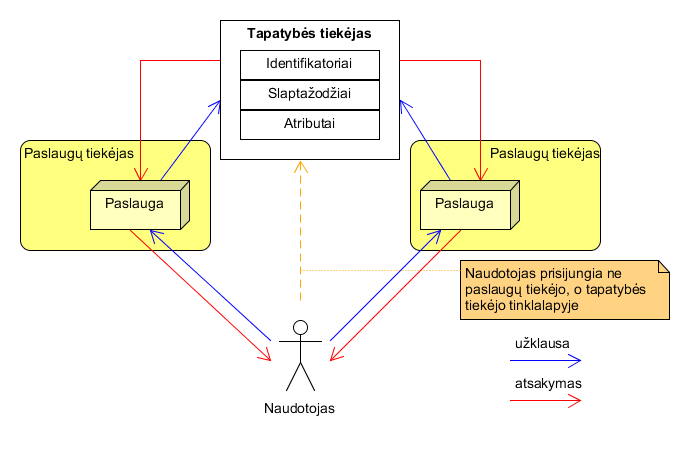
\includegraphics[scale=0.7]{img/federatedModel}
    \caption{Jungtinis skaitmeninės tapatybės valdymas \cite{Cao2010}}
    \label{fig:federatedModel}
\end{figure}

Jungtiniame tapatybės valdyme tapatybės tiekėjas yra atskira sistema, su kuria turi integruotis paslaugų tiekėjas. Tapatybės
duomenys bei su tapatybe susiję veiksmai (autentifikavimas, autorizavimas) yra deleguojami šiai sistemai. Naudotojas turi vieną identifikatorių,
su kuriuo prisijungia tiesiogiai tapatybės tiekėjo puslapyje. Prisijungus šioje sistemoje, naudotojas tampa
autentifikuotas visose paslaugose, kurios palaiko šį tapatybės tiekėją \cite{Maler2008}.

\subsubsubsection*{Realizacijos bei įgalinančios technologijos}

Kadangi jungtiniame tapatybės valdyme tapatybės tiekėjas bei paslaugų tiekėjas yra skirtingų kūrėjų sistemos,
duomenų apsikeitimui tarp jų sukurti technologiniai standartai. Trys šiuo metu labiausiai paplitę protokolai: \enquote{SAML}, \enquote{OAuth} bei \enquote{OpenID}
\cite{OIDvsOAuthvsSAML}. Šių technologijų
apžvalga pateikiama \hypertarget{tab:SSOProtocols}{~\ref{tab:SSOProtocols}}-oje lentelėje.

%Jungtinio tapatybės valdymo technologijos
%tab:SSOProtocols
% Table generated by Excel2LaTeX from sheet 'SSOProtocols'
\begin{table}[htbp]
  \centering
  \caption{Jungtinio tapatybės valdymo technologijos}
    \begin{tabular}{|p{10.22em}|p{10.11em}|p{7.945em}|p{8.78em}|}
    \hline
    \multicolumn{1}{|r|}{} & \textbf{SAML} & \textbf{OAuth} & \textbf{OpenID} \bigstrut\\
    \hline
    Dabartinė versija & SAML 2.0 & OAuth 2.0 & OpenID Connect \bigstrut\\
    \hline
    Paskirtis & Autentifikavimas, autorizavimas, atributų perdavimas & Autorizavimas & Autentifikavimas \bigstrut\\
    \hline
    Duomenų perdavimas & HTTP, SOAP & HTTP, REST & HTTP, REST \bigstrut\\
    \hline
    Duomenų formatas & XML   & JSON, JWT & JSON, JWT \bigstrut\\
    \hline
    Duomenų šifravimas & Yra   & Yra   & Yra \bigstrut\\
    \hline
    Tapatybės tiekėjo suteiktų duomenų validavimas & Viešo-privataus rakto infrastruktūra & Neapibrėžta (palikta realizacijai) & Viešo-privataus rakto infrastruktūra \bigstrut\\
    \hline
    Naudotojo sutikimas perduoti duomenis & Nėra  & Yra   & Yra \bigstrut\\
    \hline
    Mobiliųjų programėlių palaikymas & Nėra  & Yra   & Yra \bigstrut\\
    \hline
    Naudojančios organizacijos & Salesforce, PingFederate, Oracle Access Manager & Google, Amazon, GitHub & Google, Microsoft, Ping Identity \bigstrut\\
    \hline
    \end{tabular}%
  \label{tab:SSOProtocols}%
\end{table}%




Kiekviena iš minimų technologijų šiandien yra gana plačiai naudojama internete - jų svarbą parodo
ir didžiųjų kompanijų (\enquote{Google}, \enquote{GitHub}, \enquote{Microsoft}) sprendimai pritaikyti jas savo
programinėje įrangoje. Pagrindinis šių standartų skirtumas - jų panaudojimo apimtis. \enquote{SAML} pritaikytas visiems tapatybės valdymo
veiksmams, \enquote{OAuth} skirtas naudotojui autorizuoti trečiąją šalį pasiekti jo atributus tapatybės tiekėjo platformoje,
o OpenID skirtas naudotojų autentifikavimui.

\subsubsubsection*{Naudotojų poreikių įgyvendinimas}

Šis tapatybių valdymo modelis yra gana patogus naudotojams. Jis išsaugo centralizuoto modelio privalumus 
bei išplečia jo funkcionalumą už vienos organizacijos ribų \cite{OIDvsOAuthvsSAML}. Naudotojams užtenka turėti vienus atpažinimo duomenis, su kuriais
gali prisijungti prie skirtingų paslaugų tiekėjų tinklalapių. Taip pat jungtinis tapatybės valdymas turi vienkartinį prisijungimą,
kurį tinklalapyje matyti nori 77\% interneto naudotojų \cite{SSOResearch}. Vienkartinio prisijungimo pagalba naudotojui užtenka vieną kartą
prisijungti savo tapatybės tiekėjo puslapyje ir kreipiantis į visas šį tiekėją palaikančias paslaugas, jam iš naujo prisijungti nebereiks.

Asmens duomenų saugumas priklauso nuo
bendravimo tarp paslaugų bei tapatybės tiekėjų, o šiame modelyje jis sudėtingesnis nei izoliuotame ar centralizuotame
tapatybių valdyme, nes jungtinis valdymas paremtas tarpdomeniniu bendravimu \cite{Maler2008}. Saugumas sustiprinimas persiunčiamus
duomenis pasirašant taikant viešus ir privačius raktus bei užšifruojant. Tačiau, kol dauguma tinklalapių remiasi slapyvardžiu ir slaptažodžiu autentifikuojant naudotoją,
šis modelis išlieka labai pažeidžiamas sukčiavimo (angl. \textit{phishing}) atakoms \cite{Maler2008}.\\
Atliktas ne vienas tyrimas siekiant nustatyti jungtiniame tapatybės valdyme naudojamų protokolų saugumą \cite{SAMLSecurity, OAuthSecurity, OIDCSecurity}. Pripažinta, kad
sukurti automatinį protokolo saugumo analizės įrankį yra gana sunku dėl skirtingų galimų protokolų įgyvendinimo tėkmių \cite{OIDCSecurity}. Todėl jungtiniame tapatybės valdyme
naudojamų technologijų saugumas stipriai priklauso nuo konkrečių paslaugų bei tapatybės tiekėjų realizacijų detalių. Dažniausios atakos: prieigos rakto vagystės (angl. \textit{token theft}),
 apsimetimas naudotoju, sesijų apkeitimas ir specifiniai XML formato išnaudojimai, tokie kaip parašų įvyniojimas (angl. \textit{signature wrapping}) \cite{SAMLSecurity, OAuthSecurity, OIDCSecurity}.
 Šios atakos dažniausiai įgyvendinamos taikant įprastus interneto programišių metodus: XSS (angl. \textit{cross site scripting}, SQL įterpimą, puslapių apgavystes (angl. \textit{phishing}) \cite{OIDCSecurity}.

Naudotojo duomenų kontrolė jungtiniame 
modelyje turi tiek privalumų, tiek trūkumų. Viena vertus, naudotojas savo asmens duomenis suteikia mažesniam kiekiui sistemų (tik tapatybės tiekėjams,
vietoj visų paslaugų tiekėjų). Tačiau taip paslaugų tiekėjas tampa vieninteliu nesekmės tašku (angl. \textit{single point of failure}) - programišiams įsilaužus
į tapatybės tiekėjo sistemą, asmens paskyros visose paslaugose tampa prieinamos \cite{Pashalidis2003}. Taip pat, naudotojui gali būti sunku kontroliuoti
savo duomenų sklaidą tarp tapatybės tiekėjo ir skirtingų paslaugų, ką rodo ir \textit{Cambridge Analytica} incidentas \cite{CambridgeAnalytica}. Nors \enquote{OpenID Connect} bei \enquote{OAuth 2.0}
standartai suteikia galimybes naudotojui išreikštinai patvirtinti, kokius duomenis jis sutinka perduoti trečiosios šalies paslaugai, kai
jis pradeda ja naudotis (pavyzdys pateikiamas priede \hypertarget{appendix:SSOUserConsent}{~\ref{appendix:SSOUserConsent}}), tačiau tapatybės tiekėjai ne visada tinkamai informuoja,
kokie naudotojo veiksmai gali neišreikštai suteikti leidimą tapatybės tiekėjui perduoti duomenis kitai sistemai.


\subsubsection{Skaitmeninės tapatybės valdymo modelių palyginimas}

Apžvelgus skirtingas skaitmeninės tapatybės valdymo architektūras,\hypertarget{tab:IDMComparison}{~\ref{tab:IDMComparison}} lentelėje pateikiamas modelių palyginimas.
Skirtingi modeliai lyginti pagal\hypertarget{section:IDMUserNeeds}{~\ref{section:IDMUserNeeds}} skyrelyje apibrėžtus naudotojų poreikius. 

Atsižvelgus į palyginimo rezultatus, galima teigti, kad jungtinis tapatybės valdymas naudotojams yra parankesnis nei centralizuotas
ar lokalizuotas valdymas. Šie modeliai verčia naudotojus kurti ir administruoti naujas paskyras nebandytose sistemose,
prisiminti daugybę slapyvardžių bei slaptažodžių (ar silpninti saugumą naudojant tą patį slaptažodį) bei kartoti prisijungimo žingsnius,
o tai įkyri naudotojams. Pasak kompanijos \enquote{Blue Research} tyrimo, tinklalapiui prašant kurti naują paskyrą 54\% interneto naudotojų
teigia paliksiantys ar negrįšiantys į tokį puslapį, o 26\% ieškos kito panašią paslaugą teikiančio tinklalapio, nereikalaujančio naujos paskyros. 

% \caption{Skirtingų tapatybės valdymo modelių palyginimas pagal naudotojo poreikius}
% \label{tab:IDMComparison}%


  % Table generated by Excel2LaTeX from sheet 'IDMEvaluation'
\begin{table}[h]
    \centering
    \caption{Skirtingų tapatybės valdymo modelių palyginimas pagal naudotojo poreikius}
    \resizebox{\columnwidth}{!}{
        \begin{tabular}{|c|p{13.72em}|p{8em}|p{9.835em}|p{9.835em}|}
            \hline
            \multicolumn{2}{|c|}{} & \textbf{Izoliuotas} & \textbf{Centralizuotas} & \textbf{Jungtinis} \bigstrut\\
            \hline
            \multicolumn{2}{|p{18.72em}|}{\textbf{Atpažinimo duomenys}} & Kiekvienai paslaugai & Kiekvienam paslaugų tiekėjui & Kiekvienam tapatybės tiekėjui \bigstrut\\
            \hline
            \multirow{2}[4]{*}{\textbf{Patogumas}} & Prisijungimų kiekis & Tiek, kiek paslaugų & Tiek, kiek paslaugų tiekėjų & Tiek, kiek tapatybės tiekėjų \bigstrut\\
        \cline{2-5}      & Naudotojo patirties vientisumas & Yra & Yra & Nėra \bigstrut\\
            \hline
            \multirow{3}[6]{*}{\textbf{Saugumas}} & Nukreipimai (angl. redirects) & Nėra & Galimi & Yra \bigstrut\\
        \cline{2-5}      & Vienas nesėkmės taškas & Nėra & Paslaugų tiekėjo tapatybės valdymo modulis & Tapatybės tiekėjas \bigstrut\\
        \cline{2-5}      & Technologiniai standartai & Paslaugos kūrėjo nuožiūra & Paslaugų tiekėjo nuožiūra & SAML 2.0, Oauth 2.0, OpenID Connect \bigstrut\\
            \hline
            \multirow{3}[6]{*}{\textbf{Kontrolė}} & Naudotojo patvirtinimas duomenis perduodant kitai paslaugai & - & Nėra & Galimas (Oauth 2.0, OpenID Connect) \bigstrut\\
        \cline{2-5}      & Duomenų suteikimas tik jų prireikus & Tai realizavus paslaugos kūrėjui & Tai realizavus paslaugų tiekėjui & Dalinis (dar nenaudotai paslaugai prašant naudotojo patvirtinimo) \bigstrut\\
        \cline{2-5}      & Tapatybės duomenų keitimas & Kiekvienos paslaugos tinklalapyje & Kiekvieno paslaugų tiekėjo tinklalapyje & Kiekvieno tapatybės tiekėjo tinklalapyje \bigstrut\\
            \hline
            \end{tabular}%
    }
      
    \label{tab:IDMComparison}%
  \end{table}%
  
  

\subsection{Naudotojų problemų tapatybės valdyme apibendrinimas} \label{IDM:problemsSummarized}

Skaitmeninės tapatybės valdymas taikant jungtinį modelį išsprendžia nemažai problemų: sumažintas
naudotojams reikalingų paskyrų kiekis, įsimintinų slapyvardžių ir slaptažodžių gausa, apribotas
reikiamų prisijungimų kiekis. Nepaisant to, nemažai problemų naudotojams išlieka. Pagrindinės iš jų:

\begin{itemize}
    \item vienintelio nesekmės taško situacija. Jungtiniame tapatybės valdyme tapatybės tiekėjas yra vienintelis nesekmės taškas (angl. \textit{single point of failure}).
    Tapatybės tiekėjui tapus nepasiekiamam, asmuo internete nebegali naudoti visų paslaugų, kurios buvo integruotos
    su šiuo tapatybės tiekėju.

    \item kontrolės trūkumas. Organizacijos renka didžiulius kiekius asmens duomenų - \enquote{Facebook} nuo sukūrimo
    jau sukaupė 300 petabaitų duomenų apie naudotojus \cite{Vagata2014}, tačiau naudotojai nėra pakankamai informuoti,
    kur perduodami jų duomenys. Nors naudojamos technologijos, tokios kaip \enquote{OAuth}, išreikštinai prašo naudotojų
    sutikimo perduodant duomenis naujai paslaugai (žr. priedą \hypertarget{appendix:SSOUserConsent}{~\ref{appendix:SSOUserConsent}}), tai atliekama tik pradedant naudotis tam tikra paslauga. Taip pat,
    \textit{CambridgeAnalytica} incidentas \cite{CambridgeAnalytica} rodo, kad šio sutikimo gali neužtekti.
    Visa tai veda prie to, kad naudotojai jaučiasi nekontroliuojantys savo asmens duomenų internete, norėtų lengviau keisti bei trinti juos, o
    dalį tapatybės valdymo sistemų naudoja tik todėl, kad neturi kitos išeities \cite{Baars2016};

    \item pasitikėjimo stoka. Naudotojams jungtiniame tapatybės valdyme tenka pasikliauti tiek tapatybės tiekėjų,
    tiek paslaugų tiekėjų gebėjimu patikimai saugoti ir perduoti tapatybės duomenis. Norint naudotojų pasitikėjimo,
    sistemos turėtų būti skaidrios (angl. \textit{transparent}) apie tai, kaip jos saugo, valdo tapatybės duomenis \cite{Baars2016}.
    Tačiau, kai technologijų specifikacijos palieka vietos nesaugiam protokolų įgyvendinimui \cite{OAuthSecurity},
    o paslaugų tiekėjai retai atskleidžia sistemos veikimo detales \cite{Baars2016}, naudotojų pasitikėjimas senka;

    \item saugumo iššūkiai. Dėl naudojamų nukreipimų jungtinis tapatybės valdymas yra itin jautrus sukčiavimo (angl. \textit{phishing}) atakoms,
    tačiau paslaugų tiekėjai dažniausiai vis dar remiasi naudotojų gebėjimu atpažinti netikrus programišių tinklalapius, nors to nerekomenduoja tyrimai \cite{Sun2011}.
    Taip pat, jungtiniame tapatybės valdyme atsiranda vienas didelės vertės taikinys (angl. \textit{single high value target}) - tapatybės tiekėjas. Įsilaužus į jo sistemą,
    naudotojų atpažinimo duomenys gali būti pavogti ir panaudoti daugybėje skirtingų paslaugų tiekėjų sistemų.

\end{itemize}

Pateikti jungtinio tapatybės valdymo trūkumai rodo, kad tapatybės valdymo sritis vis dar yra tobulintina naudotojų atžvilgiu.
Naudotojams trūksta didesnės tapatybės duomenų kontrolės, o dėl galimų saugumo iššūkių, vieno nesekmės taško situacijos ir neatskleidžiamų
sistemų įgyvendinimo detalių, pasitikėti paslaugų bei tapatybės tiekėjais yra sudėtinga. Toliau darbe apžvelgiama blokų grandinės technologija, atkreipiant dėmesį
į jos potencialą spręsti įvardytas problemas skaitmeniniame tapatybių valdyme: vieno nesėkmės taško situaciją bei kontrolės, skaidrumo ir pasitikėjimo trūkumą.